\subsection{RTL View}
After adding your files you can check that the design is loaded correctly by opening up the RTL view. This represents your design
\begin{figure}[H]
    \centering
    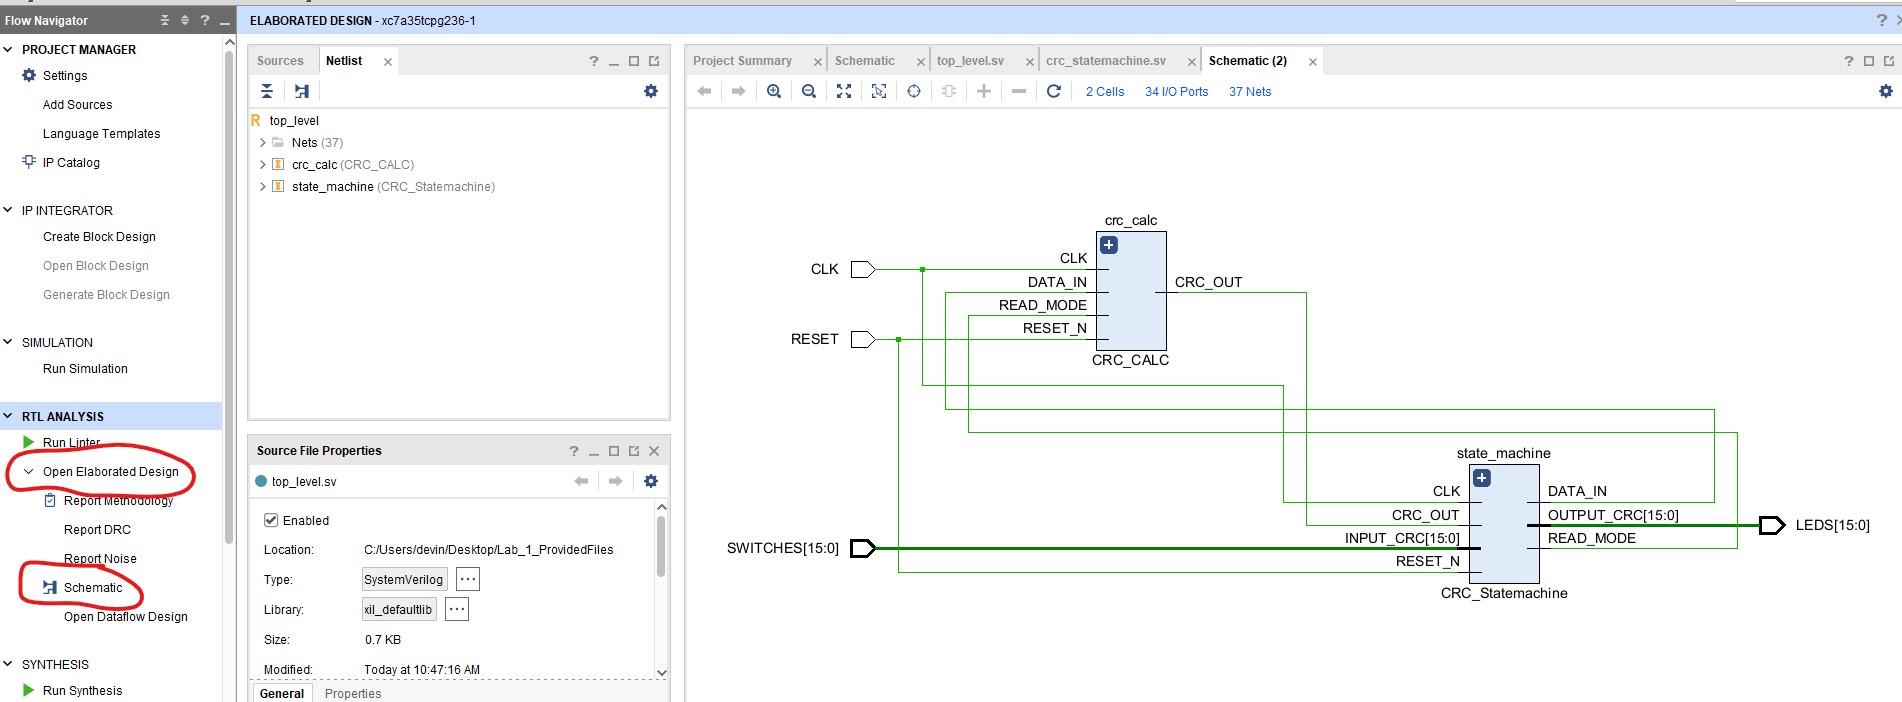
\includegraphics[width = 9cm] {Images/CreateBitstreamImages/OpenElaboratedDesign.jpg}
    \caption{Look at the RTL View}
    \label{fig:enter-label}
    \raggedright
    \vspace{0.5cm}
    Open the elaborated schematic by clicking open elaborated design, then clicking on schematic. This will compile the top level files and create a schematic representation of the design.
    You can click on the blocks in the design and it will expand out to show you the lower levels. Once finished with this lab \textbf{return to this view and include a screenshot in your design report.} Take note that no logic exists in this top level. While technically possible to have logic at any level, it is considered especially bad practice, the most logic that is considered acceptable is singular inverters. You'll need to add this to the design as part of the modifications in a later section. \\
    \vspace{0.5cm}
    
\includegraphics[height=1cm]{Images/Alert Icon.png}  \textbf{RTL view is one of the most useful tools for diagnosing problems in your FPGA design.} The RTL view represents the schematic view of your design, it is incredibly useful for confirming that you are creating the design as intended. When debugging larger designs it can be often worth restructuring larger elements to create blocks which have clear representations in the RTL view so that you can more easily diagnose issues. 
\end{figure}
\subsection{Synthesis and Implementation}
You'll remember that synthesis takes the HDL design and converts it into elements in the fpga, and then implementation takes those and maps it onto the actual fpga hardware.
\vspace{0.5cm}
\begin{figure}[H]
    \centering
    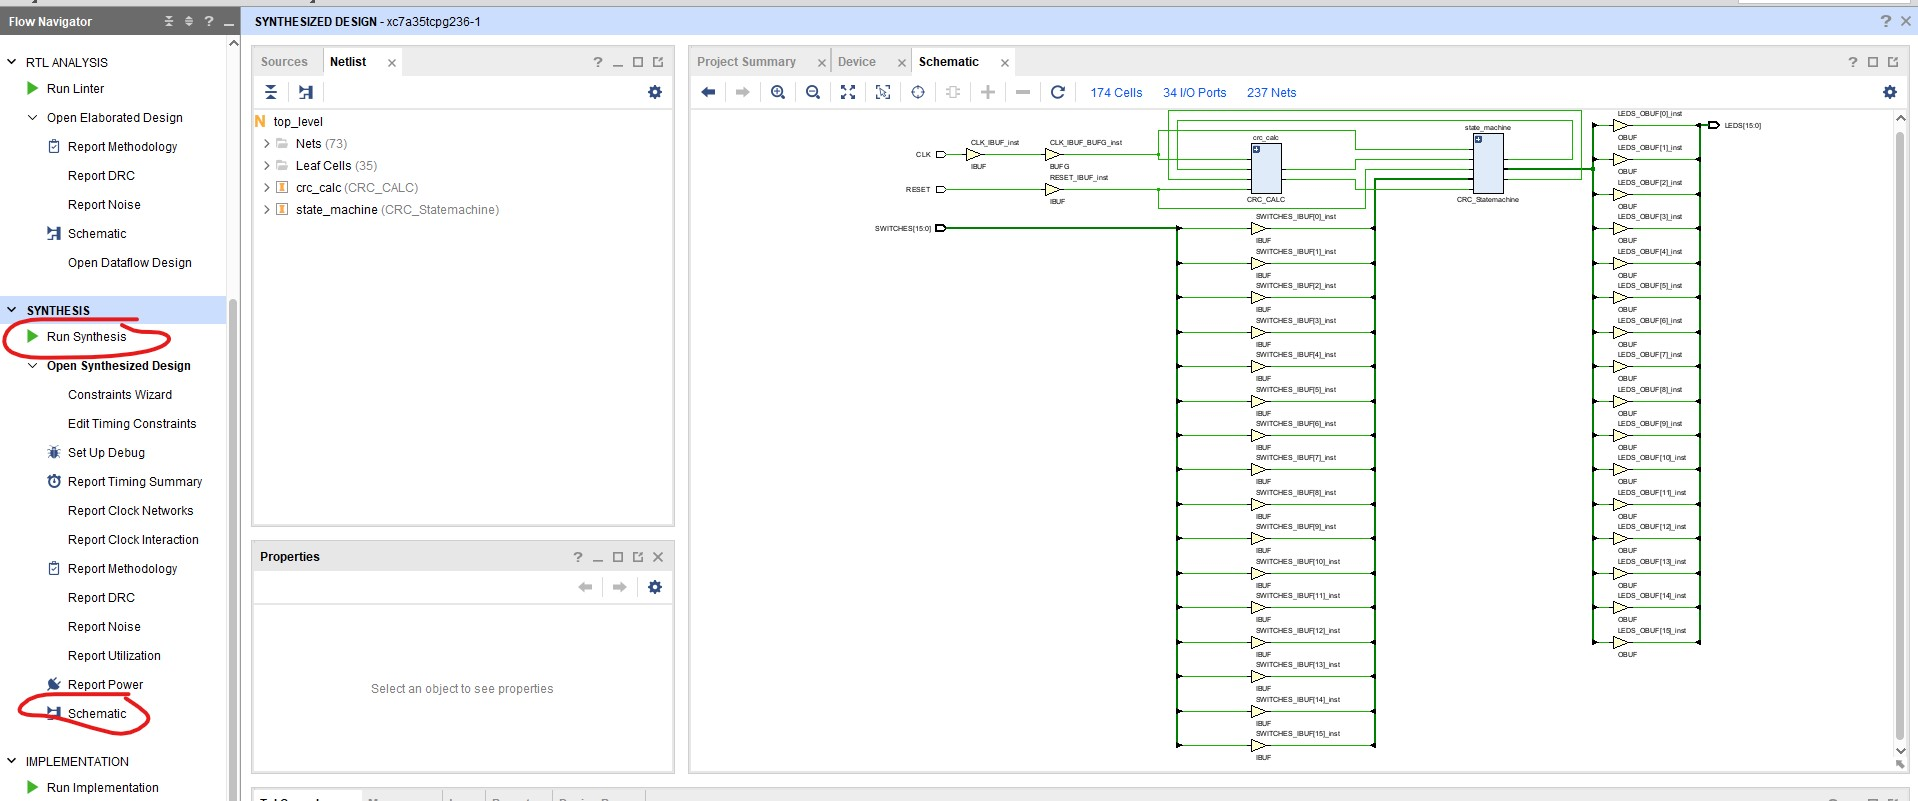
\includegraphics[width=9cm]{Images/CreateProjectImages/SynthesizeYourDesign.jpg}
    \caption{Run Synthesis}
    \label{fig:enter-label}
    \raggedright
    \vspace{0.5cm}
    Press Run Synthesis in the left hand panel. This will being up a dialog for starting synthesis, you go ahead and accept this immediately or change the number of jobs. It won't make a substantial difference in time now; however, on larger designs this will help speed up the process. Once you've run synthesis open the synthesized design and look at the schematic again, you'll notice that the logic gates have been replaced with LUTs.
\end{figure}

Once you're done looking at the elaborated design you'll want to run implementation. This will map the hardware onto the physical FPGA. This is where you'll need to grab your timing details.\\